\documentclass[border=3pt]{standalone}
% Preâmbulo compartilhado pelos diagramas TikZ da aula 4 de Navegação (Representação de Mapas)
\usepackage[T1]{fontenc}
\usepackage[utf8]{inputenc}
\usepackage{lmodern}
\usepackage{amsmath}
\usepackage{xcolor}
\usepackage{tikz}
\usetikzlibrary{arrows.meta,angles,quotes,decorations.pathmorphing,decorations.pathreplacing,calc,
                positioning,shapes.geometric,shapes.misc,backgrounds,fit,
                math}

% Paleta (mesma dos SVGs originais)
\definecolor{dblue}{HTML}{2A5B8C}
\definecolor{dorange}{HTML}{B3541E}
\definecolor{dgreen}{HTML}{4A7C59}
\definecolor{dred}{HTML}{9C4B4B}
\definecolor{dcream}{HTML}{F4F1EA}
\definecolor{dshade}{HTML}{DDD7C9}

% Função gaussiana (não normalizada por padrão de escala visual)
\pgfmathdeclarefunction{gauss}{3}{%
  \pgfmathparse{1/(#3*sqrt(2*pi))*exp(-((#1-#2)^2)/(2*#3^2))}%
}

% Estilos comuns (prefixo d... para não colidir com chaves internas do pgf)
\tikzset{
  >={Stealth[length=2mm]},
  dguide/.style={gray!55, dashed, line width=0.4pt},
  daxis/.style={gray!60, line width=0.7pt, ->},
  dbody/.style={fill=black!3, draw=black!80, line width=1pt},
  dacc/.style={draw=dblue, line width=1pt},
  dlbl/.style={black!55, font=\small},
  dsub/.style={black!45, font=\footnotesize},
  dstate/.style={circle, draw=black!80, fill=dcream, line width=1pt,
                 minimum size=17mm, font=\large, inner sep=1pt},
  dobs/.style={circle, draw=black!80, fill=dshade, line width=1pt,
               minimum size=14mm, font=\large, inner sep=1pt},
  dbox/.style={rounded corners=2pt, draw=black!80, fill=dcream, line width=1pt,
               align=center, inner sep=6pt},
  dop/.style={circle, draw=black!80, fill=white, line width=1pt,
              minimum size=6mm, inner sep=0pt, font=\small},
  dtrans/.style={->, dblue, line width=1pt},
  dmeas/.style={->, dorange, line width=1pt},
  dcurve/.style={line width=1pt, dblue},
  dcurveb/.style={line width=1.4pt, dorange},
}

\begin{document}
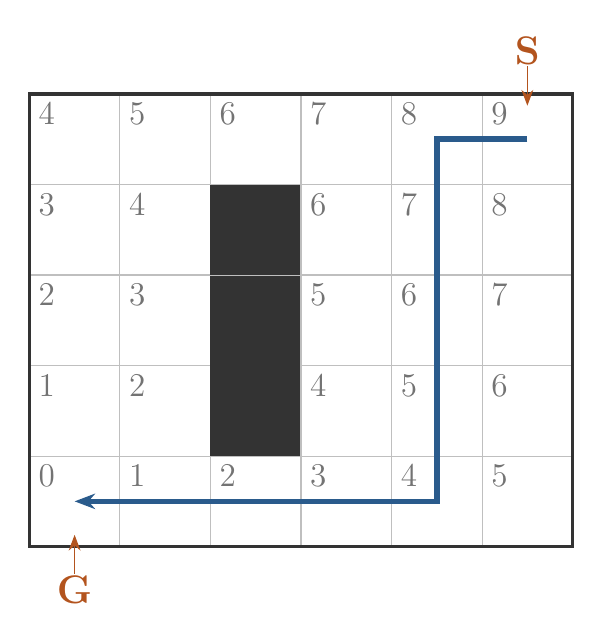
\begin{tikzpicture}[x=1cm,y=1cm]

  \def\s{1.15}

  % Grade e valores da transformada de distância (NF1 / grassfire), a partir do objetivo G
  \def\vals{{
    0,1,2,3,4,5,
    1,2,-1,4,5,6,
    2,3,-1,5,6,7,
    3,4,-1,6,7,8,
    4,5,6,7,8,9
  }}

  \foreach \row in {0,...,4} {
    \foreach \col in {0,...,5} {
      \pgfmathsetmacro{\idx}{\row*6+\col}
      \pgfmathsetmacro{\v}{\vals[\idx]}
      \pgfmathtruncatemacro{\vi}{\v}
      \draw[black!25, line width=0.4pt] (\col*\s,\row*\s) rectangle ++(\s,\s);
      \ifnum\vi<0
        \fill[black!80] (\col*\s,\row*\s) rectangle ++(\s,\s);
      \else
        \node[dlbl, font=\large, anchor=north west, inner sep=2pt] at (\col*\s+0.04,\row*\s+\s-0.04) {\vi};
      \fi
    }
  }
  \draw[draw=black!80, line width=1.2pt] (0,0) rectangle (6*\s,5*\s);

  \node[dorange, font=\bfseries\Large] at (0.5*\s,-0.55) {G};
  \draw[dorange, -{Stealth[length=2mm]}] (0.5*\s,-0.35) -- (0.5*\s,0.15);
  \node[dorange, font=\bfseries\Large] at (5.5*\s,5*\s+0.55) {S};
  \draw[dorange, -{Stealth[length=2mm]}] (5.5*\s,5*\s+0.35) -- (5.5*\s,5*\s-0.15);

  % Caminho por descida de gradiente (do maior valor até 0)
  \draw[dblue, line width=2pt, -{Stealth[length=2.6mm]}]
    (5.5*\s,4.5*\s) -- (4.5*\s,4.5*\s) -- (4.5*\s,3.5*\s) -- (4.5*\s,2.5*\s)
    -- (4.5*\s,1.5*\s) -- (4.5*\s,0.5*\s) -- (3.5*\s,0.5*\s) -- (2.5*\s,0.5*\s)
    -- (1.5*\s,0.5*\s) -- (0.5*\s,0.5*\s);

\end{tikzpicture}
\end{document}
